\documentclass{article}
\usepackage{graphicx} % Required for inserting images
\usepackage{ctex}
\usepackage{amsmath}
\usepackage{amsthm}

\theoremstyle{definition}
\newtheorem{definition}{定义}[section]

\title{Model-Free RL}
\author{Jiaqi Zheng}
\date{September 2025}

\begin{document}
\maketitle
\section{Policy Gradient(PG) Algorithm}
\par 对于强化学习问题，我们优化的目标是奖励函数的期望 $ J(\theta)=E_{\tau \sim p_{\theta}(\tau)}[\sum_t r(s_t,a_t)] $，我们希望这一函数最大化。显然，根据奖励之和的期望求出梯度是不现实的，我们希望在期望内部引入 $ \theta $，因此：
\[
 p_{\theta}(\tau)\nabla_{\theta}logp_{\theta}(\tau)=p_{\theta}(\tau)\frac{\nabla_{\theta}p_{\theta}(\tau)}{p_{\theta}(\tau)}=\nabla_{\theta}p_{\theta}(\tau)
\]
\[
 \nabla_{\theta}J(\theta)=\int \nabla_{\theta}p_{\theta}(\tau)r(\tau)d\tau=\int p_{\theta}(\tau)p_{\theta}(\tau)\nabla_{\theta}logp_{\theta}(\tau)d\tau=E_{\tau\sim p(\tau)}[p_{\theta}(\tau)\nabla_{\theta}logp_{\theta}(\tau)]
\]
\[
p_{\theta}(\tau)=p(s_1)\prod_{i=1}^T \pi_{\theta}(a_t|s_t)p(s_{t+1}|s_t,a_t)
\]
\[
logp_{\theta}(\tau)=logp(s_1)+\sum_{i=1}^Tlog\pi_{\theta}(a_t|s_t)+\sum_{i=1}^Tlogp(s_{t+1}|s_t,a_t)
\]
\[
\nabla_{\theta}J(\theta)=E_{\tau\sim p(\tau)}[(\sum_{i=1}^T\nabla_{\theta}log\pi_{\theta}(a_t|s_t))(\sum_{i=1}^Tr(s_t,a_t))]
\]
\par 于是，我们给出初步得到的Policy Gradient算法流程：
\begin{enumerate}
    \item 根据策略$ \pi_{\theta}(a_t|s_t) $采样N条轨迹
    \item 计算$ \nabla_{\theta}J(\theta)=\frac{1}{N}\sum_{i=1}^N(\sum_{i=1}^T\nabla_{\theta}log\pi_{\theta}(a_t|s_t)(\sum_{i=1}^Tr(s_t,a_t)) $
    \item 进行梯度上升$ \theta\leftarrow\theta+\alpha\nabla_{\theta}J(\theta) $
\end{enumerate}
\par 实验发现，Policy Gradient算法中无论是$ J(\theta) $还是梯度的分布均有较大的方差，这显然不利于收敛。为了减小方差，我们首先的想到的思路是增大N；其次可以减小$ J(\theta) $和梯度本身根据第二条思想，我们有以下两种思路：
\begin{enumerate}
    \item Reward-to-go
    \par 这一思路从奖励函数出发，去掉奖励函数中所有的无关部分，于是，得到的梯度为：
    \[
\nabla_{\theta}J(\theta)=E_{\tau\sim p(\tau)}[\sum_{i=1}^T\nabla_{\theta}log\pi_{\theta}(a_t|s_t)(\sum_{i=t}^Tr(s_t,a_t))]
\]
    \item Baseline
    \par 这一思路对奖励函数进行不一样的处理，我们让奖励函数减去一个常数baseline，以减小方差：
\[\nabla_{\theta}J(\theta)=E_{\tau\sim p(\tau)}[(\sum_{i=1}^T\nabla_{\theta}log\pi_{\theta}(a_t|s_t))(\sum_{i=1}^Tr(s_t,a_t)-b)]
\]
    \par 这一思路与reward-to-go可以结合使用。
\end{enumerate}
\section{Actor-Critic(AC) Algorithms}
\par 在讲Actor-Critic算法的开头，先介绍两个强化学习中的重要概念：V函数与Q函数。
\begin{definition}
    V函数指给定状态，奖励函数的期望，可以表示为：$ V(s_t)=E_{(a_t,s_{t+1},a_{t+1},s_{t+2},a_{t+2}...)\sim p_{\theta}(\tau)}[\sum_{t'=t}^Tr(s_{t'},a_{t'})] $
\end{definition}
\begin{definition}
    Q函数指给定状态和动作，奖励函数的期望。可以表示为：$ Q(s_t,a_t)=r(s_t,a_t)+E_{(s_{t+1},a_{t+1},s_{t+2},a_{t+2}...)\sim p_{\theta}(\tau)}[\sum_{t'=t+1}^Tr(s_{t'},a_{t'})] $
\end{definition}
\par 于是，Q函数与V函数存在如下关系：
\[
V(s_t)=E_{a_t\sim \pi_{\theta}(a_t|s_t)}[Q(s_t,a_t)]
\]
\[
Q(s_t,a_t)=r(s_t,a_t)+V(s_{t+1})
\]
\par 于是，我们之前得到的reward-to-go可以表示为（对于奖励函数，此刻的动作已知）：
\[
\nabla_{\theta}J(\theta)=E_{\tau\sim p(\tau)}[\sum_{i=1}^T\nabla_{\theta}log\pi_{\theta}(a_t|s_t)Q(s_t,a_t)]
\]
\par 结合上述Baseline的思想，我们将梯度表示为：
\[
\nabla_{\theta}J(\theta)=E_{\tau\sim p(\tau)}[\sum_{i=1}^T\nabla_{\theta}log\pi_{\theta}(a_t|s_t)(Q(s_t,a_t)-V(s_t))]
\]
\par 由此得到一个新的函数：优势函数。它表示某个动作相比平均值的更优程度：
\[
A^{\pi}(s_t,a_t)=Q^{\pi}(s_t,a_t)-V^{\pi}(s_t)\approx r(s_t,a_t)+V^{\pi}(s_{t+1})-V^{\pi}(s_t)
\]
\par 为了求出奖励函数，我们只需要求出V函数即可，考虑使用神经网络拟合$ V_{\phi}(s)$，其中$ \phi $为参数。
\par 在实际训练中，奖励函数的和不容易求出，因此训练数据的形式如下所示：
\[
{(s_t,r(s_t,a_t)+\hat{V}_{\phi}^{\pi}(s_{t+1})}
\]
\[
\mathcal{L}(\phi)=\frac{1}{2}\sum_i ||\hat{V}_{\phi}^{\pi}(s_{i})-y_i||^2
\]
\par 有时，为了调整不同步骤奖励的权重（更关注眼前的利益），我们引入折扣系数(Discount Factor)$ \gamma $：
\[
y_i=r(s_t,a_t)+\gamma\hat{V}_{\phi}^{\pi}(s_{t+1})
\]
\[
Q(s_t,a_t)=r(s_t,a_t)+\gamma V(s_{t+1})
\]
\[
A^{\pi}(s_t,a_t)\approx r(s_t,a_t)+\gamma V^{\pi}(s_{t+1})-V^{\pi}(s_t)
\]
\par 于是，我们初步得到了Actor-Critic算法的流程（batch）：
\begin{enumerate}
    \item 根据$ \pi_{\theta}(a|s) $对$(s_t,a_t)$进行采样。
    \item 神经网络训练$ \hat{V}_{\phi}^{\pi} $
    \item 求出$ \hat{A}^{\pi}(s_t,a_t)= r(s_t,a_t)+\gamma V^{\pi}(s_{t+1})-V^{\pi}(s_t) $
    \item $ \nabla_{\theta}J(\theta)=E_{\tau\sim p(\tau)}[\sum_{i=1}^T\nabla_{\theta}log\pi_{\theta}(a_t|s_t)\hat{A}^{\pi}(s_t,a_t)] $
    \item $ \theta\leftarrow\theta+\alpha\nabla_{\theta}J(\theta) $
\end{enumerate}
\par 现在，优势函数由两种形式：
\[
A^{\pi}_{\phi}(s_t,a_t)=r(s_t,a_t)+\gamma V_{\phi}^{\pi}(s_{t+1})-V_{\phi}^{\pi}(s_t)
\]
\[
A^{\pi}_{\phi}(s_t,a_t)=\sum_{t'=t}^{\infty}\gamma^{t'-t}r(s_{t'},a_{t'})-V_{\phi}^{\pi}(s_t)
\]
\par 前一种形式方差更小，但不是无偏估计，后一种形式是无偏估计，但是方差较大。为了结合上述两种形式的有四岸，我们提出GAE(Generalized Advantage Estimation)。考虑对上述第二个表达式进行n步截断得到：
\[
A^{\pi}_{n}(s_t,a_t)=\sum_{t'=t}^{t+n}\gamma^{t'-t}r(s_{t'},a_{t'})-V_{\phi}^{\pi}(s_t)+\gamma^n V_{\phi}^{\pi}(s_{t+n})
\]
\par 然后对不同的n进行加权求和，每一步赋予$ \lambda^n $的权重，得到：
\[
A^{\pi}_{GAE}=\sum_{n=1}^{\infty}\lambda^n A^{\pi}_{n}=\sum_{t'=t}^{\infty}(\lambda \gamma)^{t'-t}\delta_{t'}
\]
\[
\delta_{t'}=r(s_{t'},a_{t'})+\gamma V^{\pi}_{\phi}(s_{t'+1})-V^{\pi}_{\phi}(s_{t'})
\]
\par 上述策略是On-Policy的，数据来自最新的策略，这样做需要按照轨迹地对数据进行采样，效率较低。我们希望将算法改成Off-Policy的，数据来自维护的Replay Buffer，梯度下降的数据由Replay Buffer采样而来。于是，上述算法的第一步变为：根据现有策略采样动作，得到$ (s,a,s',r) $元组，将其储存到Replay Buffer中；然后从Replay Buffer中随机采样一个批次的$ (s,a,s',r) $元组。
\par 这么做会带来问题：用于梯度下降的数据不是来自于最新的策略，而V函数的目标函数是基于最新策略训练的；$ \nabla_{\theta}log\pi_{\theta}(a_t|s_t) $是基于最新策略计算的。
\par 为了解决V函数的问题，我们让目标与策略无关，考虑用Q函数代替V函数，并由训练V网络改为训练Q网络，以消除采样到旧策略对训练的影响。
\par 为了解决策略梯度的问题，我们用最新策略采样得到的动作$ a_i^{\pi} $替代Replay Buffer中的$ a_i $。
\par 于是，算法流程变成了：
\begin{enumerate}
    \item 根据现有策略采样动作，得到$ (s,a,s',r) $元组，加入Replay Buffer
    \item 从Replay Buffer中随机采样一个批次的$ (s,a,s',r) $元组。
    \item 更新$ \hat{Q}_{\phi}^{\pi}(s_t,a_t) $
    \item $ \nabla_{\theta}J(\theta)=\frac{1}{N}\sum_i \nabla_{\theta}log\pi_{\theta}(a_i^{\pi}|s_i)\hat{Q}_{\phi}^{\pi}(s_i,a_i^{\pi}) $
    \item $ \theta\leftarrow\theta+\alpha\nabla_{\theta}J(\theta) $
\end{enumerate}
\section{Q-Learning}
\par 现在，我们的想法是完全放弃对策略网络进行的优化，只对V函数、Q函数或A函数进行优化。对于策略，我们简单地选择argmax，当然，这种想法仅局限于离散动作空间。
\par 我们首先考虑一种较为简单的情况：状态空间较小，在这种情况中，可以通过动态规划(Dynamic Programming)的思想进行求值。具体步骤如下，需要注意的是，当策略改进之后需要重新进行策略迭代(Policy Iteration)：
\begin{enumerate}
    \item 对于每个状态，循环执行下面的式子，直至前后的差小于一定的值。
    \[
    V^{\pi}\leftarrow r(s,\pi(s))+\gamma E_{s'\sim p(s'|s,\pi(s))}[V^{\pi}(s')]
    \]
    \item 根据argmax改进策略
    \[
    \pi'(a_t|s_t)=\begin{cases}
    1 & \text{if}  \space a_t=argmax_{a_t}A^{\pi}(s_t,a_t) \\
    0 & \text{otherwise} \\
    \end{cases}
    \]
\end{enumerate}
\par 策略是根据argmax更新的，那么我们可以优化Q以代替V来进行，然后直接根据Q函数更新动作。于是我们得到了值迭代(Value Iteration)，即循环执行$ Q(s,a)\leftarrow r(s,a)+\gamma E[V(s')] $以及$ V(s)\leftarrow max_a Q(s,a) $。
\par 在实际情况中，状态空间巨大，应用动态规划占用大量的计算资源，于是可以考虑使用神经网络拟合。采用Actor-Critic算法中的思路：
\begin{enumerate}
    \item 训练目标（最大化的Q函数，因为我们希望V函数尽可能地大） $ y_i\leftarrow max_{a_i} (r(s_i,a_i)+\gamma E[V_{\phi}(s')]) $
    \item $ \phi \leftarrow argmin_{\phi}\frac{1}{2}\sum_i ||V_{\phi}(s_i)-y_i||^2 $
\end{enumerate}
\par 这种算法需要知道转移状态(Transition Dynamics)，即在一定状态下，一定动作会把我们带去什么地方，而转移状态并不是对每个环境都十分清楚的，由此，我们再次使用之前的max trick，对Q函数进行拟合：
\begin{enumerate}
    \item 训练目标 $ y_i\leftarrow r(s_i,a_i)+\gamma max_{a'}Q_{\phi}(s_i',a_i') $
    \item $ \phi \leftarrow argmin_{\phi}\frac{1}{2}\sum_i ||Q_{\phi}(s_i,a_i)-y_i||^2 $
\end{enumerate}
\par 由于输入数据是$ (s,a) $二元组，与策略无关，因此可以引入Replay Buffer，其内部数据结构为$ (s,a,r,s') $。在循环进行一定次数之后定期根据最新策略(argmax)向Replay Buffer中添加数据。
\par 基础的Q-Learning算法就是由上述算法改进而来，为了节约计算资源，其中每次得到目标之后只进行一次梯度下降（因为目标并不精准）。
\par 这一算法是off-policy的，$ (s,a) $二元组并不是通过最新的策略产生的。对于最终策略的选择，除了最简单的argmax方法，还有：
\begin{enumerate}
    \item epsilon-greedy:
    \[
    \pi(a_t|s_t)=\begin{cases}
    1-\epsilon & \text{if}  \space a_t=argmax_{a_t}Q_{\phi}(s_t,a_t) \\
    \epsilon/(|\mathcal{A}-1|) & \text{otherwise} \\
    \end{cases}
    \]
    \item Boltzmann Exploration
    \[
    \pi(a_t|s_t)\propto exp(Q_{\phi}(s_t,a_t))
    \]
\end{enumerate}
\par Q-Learning中为了节约计算资源，每次得到目标之后只进行一次梯度下降。但是这样优化的是一个时时刻刻在移动的目标，不利于模型的收敛，由此，我们对目标函数入手，希望在迭代一定步骤之内目标不变，于是有了Target Network。
    \begin{figure}[h]
        \centering
        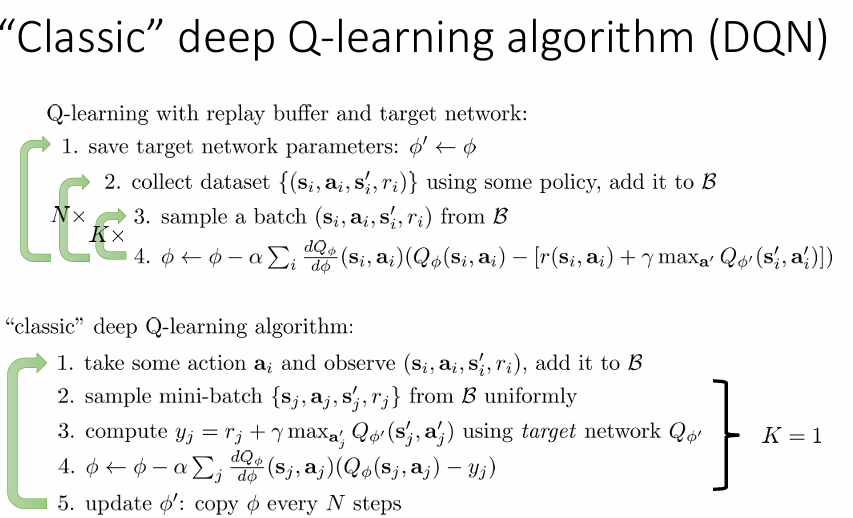
\includegraphics[width=0.6\textwidth]{DQN.png} 
        \caption{Deep Q-Learning}
        \label{fig:example}
    \end{figure}

\par 对于Target Network的更新问题，我们可以选择Polyak Averaging使得更新更加平滑，即：
\[
\phi'\leftarrow \tau\phi'+(1-\tau)\phi\space,\space\tau=0.999\space \text{works well}
\]
\par 我们通过上述算法得到的Q函数不是无偏的，在确定目标值的计算中，max操作倾向于选择被高估的动作对应的Q，从而导致Q被高估，这种高估不断地传递下去会对结果产生较大的影响。从数学上讲，由于$ E[max(X_1,X_2)]\geq max(E[X_1],E[X_2]) $，max操作求的是最大值的期望，因此会存在高估。
\par 对于这种问题，我们引入了Double Q-Learning，这样可以及时地对高估进行纠正。训练目标如下所示：
\[
Q_{\phi_A}\leftarrow r+\gamma Q_{\phi_B}(s',argmax_{a'}Q_{\phi_A}(s',a'))
\]
\[
Q_{\phi_B}\leftarrow r+\gamma Q_{\phi_A}(s',argmax_{a'}Q_{\phi_B}(s',a'))
\]
\par 实验证明，这种思路效果很好，如下图所示：
    \begin{figure}[h]
        \centering
        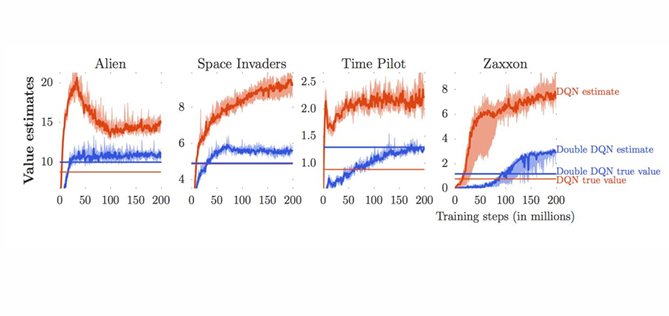
\includegraphics[width=0.6\textwidth]{DDQN.png} 
        \caption{Deep Q-Learning}
        \label{fig:example}
    \end{figure}
\end{document}
